\documentclass[11pt,a4paper]{ctexart}
% 调整页面大小,默认页面与常用规格不符
\usepackage[margin=1in,top=1.5in]{geometry}
\pagestyle{headings}
\usepackage[utf8]{inputenc}

\usepackage{float}

% 插入数学及电学符号
\usepackage{amsmath}
\usepackage{amsfonts}
\usepackage{amssymb}

% 插入附件
%\usepackage{navigator}

% 引用链接可点击
\usepackage{cite}
\usepackage[colorlinks,linkcolor=black,anchorcolor=blue,citecolor=green]{hyperref}

% 插入图片
\usepackage{graphicx}

% 绘制各种图形,包括电路图,函数图
\usepackage{tikz}
\usepackage{pgfplots}

\makeatletter
\newcommand\dlmu[2][4cm]{\hskip1pt\underline{\hb@xt@ #1{\hss#2\hss}}\hskip3pt}
\makeatother

% 标题居左 显示成如下情况 一、标题
\ctexset{
	section={
		name={第,章},
		number=\arabic{section},
		format=\Large\bfseries\raggedright\heiti
	},
}

% 设置页眉
\usepackage{fancyhdr}
\pagestyle{fancy}
\fancyhf{} % 清空当前的页眉页脚
\fancyhead[C]{\heiti 计算机系统实验报告}

% 用于插入C代码
\usepackage{minted}

\bibliographystyle{plain}
\numberwithin{figure}{section}

\begin{document}
\heiti
\begin{titlepage}
	\centering
	\rule[1.10cm]{\linewidth}{0cm}
	
	
\includegraphics[width=0.4\linewidth]{../Banner}
	
	\vspace{0.5cm}
	\textbf{\zihao{0} 实验报告}
	
	\vspace{1cm}
	\textbf{{\Huge 实验(一)}}
	
	\begin{LARGE}
		\vspace{2cm}
		题\rule{38pt}{0pt}目 \dlmu[6cm]{Linux下C工具应用} \\ \vspace{4pt}
		专\rule{38pt}{0pt}业 \dlmu[6cm]{计算机系} \\ \vspace{4pt}
		学\rule{38pt}{0pt}号 \dlmu[6cm]{1160300202}\\ \vspace{4pt}
		班\rule{38pt}{0pt}级 \dlmu[6cm]{1603002}\\ \vspace{4pt}
		学\rule{38pt}{0pt}生 \dlmu[6cm]{冯云龙}\\ \vspace{4pt}
		指导教师 \dlmu[6cm]{刘宏伟}\\ \vspace{4pt}
		实验地点 \dlmu[6cm]{G712}\\ \vspace{4pt}
		实验日期 \dlmu[6cm]{2017/10/10}\\ \vspace{4pt}
	\end{LARGE}
	
	\vfill
	{\huge \textbf{计算机科学与技术学院}}% 底部插入当日日期
\end{titlepage}

\tableofcontents
\newpage
\section{实验基本信息}

\subsection{实验目的}
\begin{enumerate}
	\item 运用现代工具进行计算机软硬件系统的观察与分析
	\item 运用现代工具进行Linux下C语言的编程调试
	\item 初步掌握计算机系统的基本知识与各种类型的数据表示
\end{enumerate}

\subsection{实验环境与工具}

\subsubsection{硬件环境}
\begin{itemize}
	\item CPU: Intel Core i7-6700HQ @ 8x 3.5GHz
	\item RAM: 3516MiB / 7899MiB
\end{itemize}

\subsubsection{软件环境}
\begin{itemize}
	\item Manjaro Linux

\end{itemize}

\subsubsection{开发工具}
\begin{itemize}
	\item Virtual BOX
	\item GCC
	\item Clion
\end{itemize}

\subsection{实验预习}

\begin{itemize}
	\item 在Windows下编写hellowin.c,显示“Hello\ 1160300202冯云龙” %可用VI、VIM、EMACS、GEDIT等,换成学生自己信息
	\item 在Linux下编写hellolinux.c,显示“Hello\ 1160300202冯云龙” %可用VI、VIM、EMACS、GEDIT等,换成学生自己信息
	\item 编写showbyte.c,以16进制显示文件hello.c等的内容:每行16个字符,上一行为字符,下一行为其对应的16进制形式。
	\item 编写datatype.c,定义C所有类型的全局变量,并赋初值。%如整数可以是学号(数字部分),字符串可以是你的姓名,浮点数可以是身份证号的数字部分。主程序打印每个变量的变量名、变量值、变量地址、变量对应16进制的内存各字节。
\end{itemize} %实验基本信息
\section{预备知识}

\subsection{给出ISA+的指令编码设计}

\begin{table}[H]
    \centering
    \begin{tabular}{|c|c|c|c|c|c|c|c|c|c|c|}
        \hline 
        字节 & 0 & 1 & 2 & 3 & 4 & 5 & 6 & 7 & 8 & 9 \\ 
        \hline 
        halt & 0|0 & \multicolumn{9}{c|}{} \\ 
        \hline 
        nop & 1|0 & \multicolumn{9}{c|}{} \\ 
        \hline 
        rrmovq rA,rB & 2|0 & rA|rB & \multicolumn{8}{c|}{} \\ 
        \hline 
        irmovq V,rB & 3|0 & F|rB & \multicolumn{8}{c|}{V} \\ 
        \hline 
        rmmovq rA,D(rB) & 4|0 & rA,rB & \multicolumn{8}{c|}{D} \\ 
        \hline 
        mrmovq D(rB),rA & 5|0 & rA,rB & \multicolumn{8}{c|}{D} \\ 
        \hline 
        OPq rA,rB & 6|fn & rA,rB & \multicolumn{8}{c|}{} \\ 
        \hline 
        jXX Dest & 7|fn & \multicolumn{8}{c|}{Dest} &  \\ 
        \hline 
        cmovXX rA,rB & 2|fn & rA,rB & \multicolumn{8}{c|}{} \\ 
        \hline 
        call Dest & 8|0 & \multicolumn{8}{c|}{Dest} &  \\ 
        \hline 
        ret & 9|0 & \multicolumn{9}{c|}{}  \\ 
        \hline 
        pushq rA & A|0 & rA|F & \multicolumn{8}{c|}{} \\ 
        \hline 
        popq rA & B|0 & rA|F & \multicolumn{8}{c|}{} \\ 
        \hline 
        iaddq V,rB & C|0 & F|rB & \multicolumn{8}{c|}{V} \\ 
        \hline 
    \end{tabular} 
    \caption{ISA+指令集}
\end{table}

\begin{table}[H]
    \centering
   \begin{tabular}{|c|c|c|c|c|c|c|c|c|c|}
       \hline 
       \multicolumn{2}{|c|}{整数操作指令} & \multicolumn{4}{|c|}{分支命令} & \multicolumn{4}{|c|}{传送指令} \\ 
       \hline 
       addq & 6|0 & jmp & 7|0 & jne & 7|4 & rrmovq & 2|0 & cmovne & 2|4 \\ 
       \hline 
       subq & 6|1 & jle & 7|1 & jge & 7|5 & cmovle & 2|1 & cmovge & 2|5 \\ 
       \hline 
       andq & 6|2 & jl & 7|2 & jg & 7|6 & cmovl & 2|2 & cmovq & 2|6 \\ 
       \hline 
       xorq & 6|3 & je & 7|3 &  &  & cmove & 2|3 &  &  \\ 
       \hline 
   \end{tabular} 
   \caption{ISA+指令集功能码}
\end{table}

\begin{table}[H]
    \centering
    \begin{tabular}{|c|c|c|c|c|c|c|c|c|}
        \hline 
        数字 & 0 & 1 & 2 & 3 & 4 & 5 & 6 & 7  \\ 
        \hline 
        寄存器名字 & \%rax & \%rcx & \%rdx & \%rbx & \%rsp & \%rbp & \%rsi & \%rdi  \\ 
        \hline 
        数字 & 8 & 9 & A & B & C & D & E & F \\
        \hline
        寄存器名字 & \%r8 & \%r9 & \%r10 & \%r11 & \%r12 & \%r13 & \%r14 & 无寄存器 \\
        \hline
    \end{tabular} 
    \caption{ISA+寄存器标识符}
\end{table}

\subsection{写出指令iaddq在SEQ中的计算过程}

\begin{enumerate}
    \item 取指令(Fetch)
    \subitem icode:ifun = M1[PC]
    \subitem rA:rB=M1[PC+1]
    \subitem valC=M8[PC+2]
    \subitem valP=PC+10
    \item 译码(Decode)
    \subitem valB=R[rB]
    \item 执行(Excute)
    \subitem valE=valB + valC
    \subitem set CC
    \item 写回(Memory)
    \item 更新PC(Write)
    \subitem R[rB]=valE
\end{enumerate}

\subsection{使用iaddq指令重写教材图4-6中的sum函数}

\begin{minted}{gas}
sum:
    xorq   %rax,%rax
    andq   %rsi,%rsi
    jmp    test
loop:
    mrmovq (%rdi),%r10
    addq   %r10,%rax
    iaddq  $8,%rdi
    iaddq  $-1,%rsi
test:
    jne loop
    ret
\end{minted}


 %实验环境建立
\section{Y86-64顺序处理器设计}
\begin{center}
    (该章满分50分)
\end{center}

\subsection{Y86-64顺序处理器结构设计}

\begin{figure}[H]
\centering
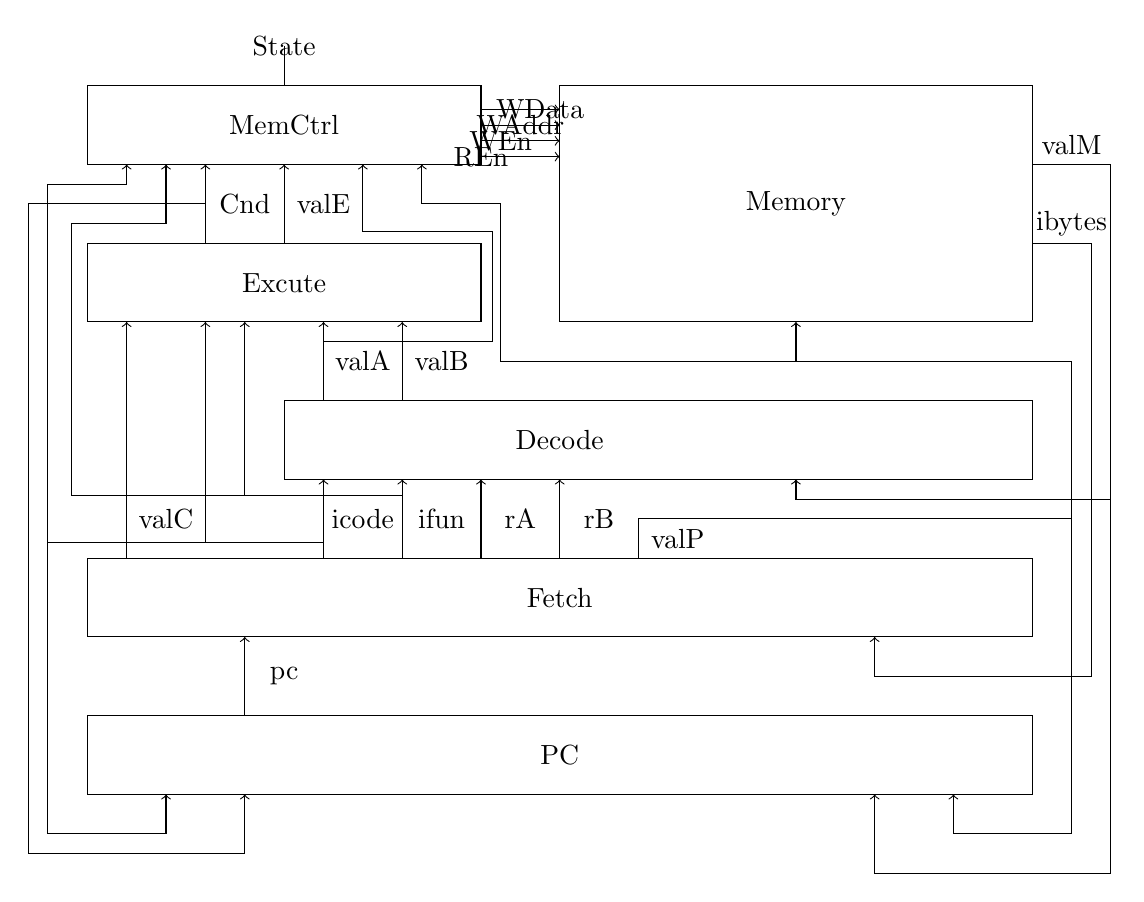
\begin{tikzpicture}
    \draw (0,0) rectangle +(12,1);
    \draw (6,0.5) node{PC};
    
    \draw (0,2) rectangle +(12,1);
    \draw (6,2.5) node{Fetch};
    
    \draw (2.5,4) rectangle +(9.5,1);
    \draw (6,4.5) node{Decode};
    
    \draw (0,6) rectangle +(5,1);
    \draw (2.5,6.5) node{Excute};
    
    \draw (0,8) rectangle +(5,1);
    \draw (2.5,8.5) node{MemCtrl};
    
    \draw (6,6) rectangle +(6,3);
    \draw (9,7.5) node{Memory};

%pc
    \draw [->](2,1) -- (2,2);
    \draw (2.5,1.5) node{pc};
    
%fetch
    \draw [->](3,3) -- (3,4);
    \draw [->](3,3.2) -- (1.5,3.2) -- (1.5,6);
    \draw [->](3,3.2) -- (-0.5,3.2) -- (-0.5,-0.5) -- (1,-0.5) -- (1,0);
    \draw [->](-0.5,3.2) -- (-0.5,7.75) -- (0.5,7.75) -- (0.5,8);
    \draw (3.5,3.5) node{icode};
    
    \draw [->](4,3) -- (4,4);
    \draw [->](4,3.8) -- (2,3.8) -- (2,6);
    \draw [->](4,3.8) -- (-0.2,3.8) -- (-0.2,7.25) -- (1,7.25) -- (1,8);
    \draw (4.5,3.5) node{ifun};
    
    \draw [->](5,3) -- (5,4);
    \draw (5.5,3.5) node{rA};
    
    \draw [->](6,3) -- (6,4);
    \draw (6.5,3.5) node{rB};
    
    \draw [->](0.5,3) -- (0.5,6);
    \draw (1,3.5) node{valC};
    
    \draw [->](7,3) -- (7,3.5) -- (12.5,3.5) -- (12.5,3.5) -- (12.5,-0.5) -- (11,-0.5) -- (11,0);
    \draw [->](12.5,3.5) -- (12.5,5.5) -- (5.25,5.5) -- (5.25,7.5) -- (4.25,7.5)--(4.25,8);
    \draw [->](9,5.5)--(9,6);
    \draw (7.5,3.25) node{valP};
    
%decode
    \draw [->](3,5) -- (3,6);
    \draw [->](3,5.75) -- (5.15,5.75) -- (5.15,7.15) -- (3.5,7.15) -- (3.5,8);
    \draw (3.5,5.5) node{valA};
    
    \draw [->](4,5) -- (4,6);
    \draw (4.5,5.5) node{valB};
    
%execute
    \draw [->](1.5,7) -- (1.5,8);
    \draw [->](1.5,7.5) -- (-0.75,7.5) -- (-0.75,-0.75) -- (2,-0.75) --(2,0);
    \draw (2,7.5) node{Cnd};
    
    \draw [->](2.5,7) -- (2.5,8);
    \draw (3,7.5) node{valE};
    
%memctrl
    \draw [->] (5,8.1) -- (5.0,8.1)node{REn} -- (6,8.1);
    \draw [->] (5,8.3) -- (5.25,8.3)node{WEn} -- (6,8.3);
    \draw [->] (5,8.5) -- (5.5,8.5)node{WAddr} -- (6,8.5);
    \draw [->] (5,8.7) -- (5.75,8.7)node{WData} -- (6,8.7);
    \draw (2.5,9) -- (2.5,9.5) node{State};
    
%memory
    \draw [->] (12,7) -- (12.75,7) -- (12.75,1.5) -- (10,1.5)--(10,2);
    \draw (12.5,7.25) node{ibytes};
    \draw [->] (12,8) -- (13,8) -- (13,-1) --(10,-1) -- (10,0);
    \draw [->] (13,3.75)--(9,3.75)--(9,4);
    \draw (12.5,8.25)node{valM};

\end{tikzpicture}
\caption{Y86-64处理器结构}
\end{figure}

\subsection{Y86-64顺序处理器模块设计(包含Verilog模块接口设计)}

\subsubsection{PC}
\begin{minted}{verilog}
module PC(
    input clock,
    input  [3:0] icode,
    input  Cnd,
    input  [63:0] ValM,
    input  [63:0] ValC,
    input  [63:0] ValP,
    output reg[63:0] pc,
    input reset
);
\end{minted}

根据icode和cnd对PC进行更新。

\subsubsection{取指}
\begin{minted}{verilog}
module Fetch(
    input [63:0] pc,
    input [79:0] ibytes,
    input imem_error,
    output instr_valid,
    output [3:0] icode,
    output [3:0] ifun,
    output [3:0] rA,
    output [3:0] rB,
    output [63:0] valC,
    output [63:0] valP
);
\end{minted}

对传入的ibytes进行解析,拆分成icode,ifun,rA,rb,valC,并根据拆分值计算valP。


\subsubsection{译码}
\begin{minted}{verilog}
module Decode(
    input clock,
    input [3:0] icode,
    input [3:0] rA,
    input [3:0] rB,
    input cnd,
    input [63:0] valM,
    input [63:0] valE,
    output [63:0] valA,
    output [63:0] valB
);
\end{minted}

传入rA、rB、icode、Cnd,根据icode的值和Cnd的值读出寄存器的值并对寄存器文件进行写入。

\subsubsection{执行}
\begin{minted}{verilog}
module Excute(
    input clock,
    input  [3:0] icode,
    input  [3:0] ifun,
    input  [63:0]valC,
    input  [63:0]valA,
    input  [63:0]valB,
    input  reset,
    output Cnd,
    output [63:0]valE
);
\end{minted}

根据指令icode进行数据运算,并更新Cnd。

\subsubsection{访存}
\begin{minted}{verilog}
module MemCtrl(
    input [3:0]icode,
    input [63:0]valE,
    input [63:0]valA,
    input [63:0]valP,
    input instr_valid,
    input im_error,
    input dm_error,
    output readEn,
    output writeEn,
    output [1:0]status,
    output [63:0]mem_addr,
    output [63:0]mem_data
);
\end{minted}

根据icode的值决定内存读信号和内存写信号,以及内存地址的取值和写入内存的数据。该模块与Bmemory模块连接,控制内存的读写,同时输出处理器运行状态。

\begin{minted}{verilog}
module BMemory(
    input clock,
    input read,
    input write,
    input [63:0] maddr,
    input [63:0] wdata,
    output [63:0] rdata, //valM
    input [63:0] iaddr,
    output [79:0] idata,
    output i_ok,
    output m_ok
);
\end{minted}

根据内存控制信号执行相应操作。如果内存读信号为1,则通过内存地址按字节依次取出该数据存入寄存器,如果内存写信号为1,则把要写入内存的数据写入内存。

\subsubsection{处理器}
\begin{minted}{verilog}
module Processor(
    input [2:0] mode,
    input [63:0] udaddr,
    input [63:0] idata,
    input clock
);
\end{minted}

对各个模块进行综合,形成完整的处理器,这里可以通过改变状态对内存进行读写操作。
 %WINDOWS软硬件系统观察与分析
\section{设计验证}
\begin{center}
    (该章满分20分)
\end{center}

\subsection{仿真验证}

选取2.3节中的任意两条机器指令,给出机器码格式,建立testbench文件,进行波形仿真。给出测试结果(波形图需要截屏)。

这里所给出的Processor已经被修改过了,主要是为了可以直观的看到执行机器码之后对寄存器的修改。

\begin{minted}{gas}
30f20a00000000000000 |   irmovq $10,%rdx
30f00300000000000000 |   irmovq  $3,%rax
6020                 |   addq %rdx,%rax
\end{minted}

\begin{minted}{verilog}
module testbench( );
    parameter RUN_MODE = 2'h0;
    parameter RESET_MODE = 2'h1;
    parameter DOWNLOAD_MODE = 2'h2;
    parameter UPLOAD_MODE = 2'h3;
    
    reg clock = 0;
    reg [2:0] mode = RESET_MODE;
    reg [63:0]uaddr = 0;
    reg [63:0]idata = 1;
    wire [63:0]rax;
    wire [63:0]rdx;
    
    always begin
        clock = 1;
        # 5;
        clock = 0;
        # 5;
    end
    
    //30f20a00000000000000 |   irmovq $10,%rdx
    //30f00300000000000000 |   irmovq  $3,%rax
    //6020                 |   addq %rdx,%rax
    
    initial begin
    #20 mode <= DOWNLOAD_MODE;
    uaddr <= 0;
    idata <= 64'h00000000000af230;
    #20;
    uaddr <= 8;
    idata <= 64'h00000003f0300000;
    #20;
    uaddr <= 16;
    idata <= 64'h000206000000000;
    #20;
    uaddr <= 24;
    idata <= 64'h0000000000000000;
    #20 mode <= RESET_MODE;
    #20 mode <= RUN_MODE;
    end
    
    Processor p(mode,uaddr,idata,rax,rdx,clock);

endmodule
\end{minted}

\begin{figure}
    \centering
    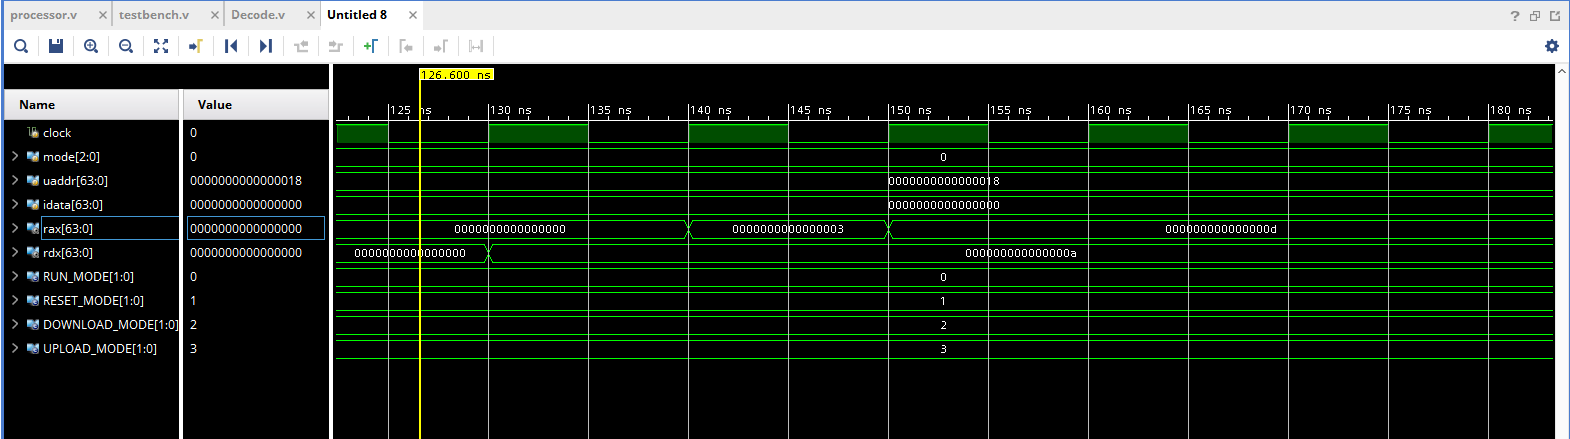
\includegraphics[width=0.7\linewidth]{figures/Sim}
    \caption{仿真波形}
    \label{fig:sim}
\end{figure}


\subsection{综合(synthesis)验证}
\begin{center}
    (选做,加分项,最多加分值为作业项总成绩的5分,作业项分值加满为止)
\end{center}

以2.3节中的程序为例,写出对应机器码格式,在某FPGA实验台上验证。

\section{总结}
\subsection{请总结本次实验的收获}
\begin{enumerate}
    \item 重新复习了vivado和verilog相关知识
    \item 对CPU顺序处理器的内部结构和运转过程有了更加深入的了解
    \item 在对SEQ不断修改调整的过程中加深了对CPU功能及与内存关系的理解
\end{enumerate}

\subsection{请给出对本次实验内容的建议}
希望可以第一时间给出参考资料。 %LINUX软硬件系统观察与分析
\section{以16进制查看程序HELLO.C}
\subsection{请查看HELLOWIN.C与HELLOLINUX.C的编码(3分)}

HelloWin.c采用\dlmu[2cm]{GBK}编码,HelloLinux.c 采用\dlmu{UTF-8}编码,你的姓名\dlmu[2cm]{冯云龙}分别编码为:\dlmu[7cm]{B7\ EB\ D4\ C6\ C1\ FA}\\
与\dlmu[7cm]{E5\ 86\ AF\ E4\ BA\ 91\ E9\ BE\ 99\ 0A}。

HelloWin.c在Linux下用gcc缺省模式编译后运行结果为:\dlmu[5cm]{Hello\ 1160300202\ ??????}。

\subsection{请查看HELLOWIN.C与HELLOLINUX.C的回车(3分)} 

Windows下的回车编码为:\dlmu[2cm]{0D\ 0A},Linux下的回车编码为:\dlmu[2cm]{0A 0A}。
交叉打开文件的效果是\dlmu[6cm]{hellolinux.c全部变成一行},
\dlmu[6cm]{hellowin.c 后面多了一个 $\hat{ } M$ 符号}。

\section{程序的生成CPP、GCC、AS、LD}

%\subsection{请提交每步生成的文件(4分)}
%\embeddedfile[Source file]{hellolinux.c}{src/hello.c}
%\embeddedfile[Preprocess file]{hellolinux.i}{src/hello.o}
%\embeddedfile[Assemble file]{hellolinux.o}{src/hello.c}
%\embeddedfile[Object file]{hellolinux.out}{src/hello.out}

\begin{enumerate}
	\item 预处理,生成预编译文件(.i文件):\mintinline{sh}|Gcc –E hello.c –o hello.i|
	\item 编译,生成汇编代码(.s文件):\mintinline{sh}|Gcc –S hello.i –o hello.s|
	\item 汇编,生成目标文件(.o文件):\mintinline{sh}|Gcc –c hello.s –o hello.o|
	\item 链接,生成可执行文件:\mintinline{sh}|Gcc hello.o –o hello.out|
\end{enumerate}

\inputminted{c}{src/hello.c}

%需要提交的文件在PDF附件当中。 %以16进制查看程序HELLO.C %程序的生成
\section{计算机系统的基本信息获取编程}
\subsection{CPUID信息}
CPUID指令是intel IA32架构下获得CPU信息的汇编指令,可以得到CPU类型,型号,制造商信息,商标信息,序列号,缓存等一系列CPU相关的东西。
cpuid使用eax作为输入参数,eax,ebx,ecx,edx作为输出参数。

把eax = 0作为输入参数,cpuid指令执行以后,会返回一个12字符的制造商信息,前四个字符的ASCI码按低位到高位放在ebx,中间四个放在edx,最后四个字符放在ecx。
把eax = 1作为输入参数,cpuid指令执行以后,会返回CPU的版本、架构和签名,签名信息放在eax,特性放在edx和ecx,附加特性放在ebx。

\subsection{获取MAC}
使用\mintinline{c}|ioctl|和\mintinline{c}|socket|函数获取网卡MAC地址。

socket函数用于创建套接字,之后我们使用这个套接字来获取网卡的MAC地址,I/O控制函数ioctl用于对文件进行底层控制,这里的文件包含网卡、终端、磁带机、套接口等软硬件设施,实际的操作来自各个设备自己提供的ioctl接口。

\mintinline{c}|int socket(int domain,int type, int protocol);|
\begin{itemize}
	\item domain参数:表示所使用的协议族(取值AF\_INET,表示采用internet协议族)
	\item type参数:表示套接口的类型(SOCK\_DGRAM,表示采用数据报类型套接口)
	\item protocol参数:表示所使用的协议族中某个特定的协议(自动选择,用0填充)
\end{itemize}

如果函数调用成功,套接口的描述符(非负整数)就作为函数的返回值,假如返回值为-1,就表明有错误发生。

\mintinline{c}|int ioctl(int fd,int request,…)|。
\begin{itemize}
	\item fd参数:文件描述符(取套接口的描述符)
	\item request参数:指定信息获取码(SIONGIFHWADDR表示取硬件地址)
	\item 其后的request参数用于为实现I/O控制所必须传入或传出的参数
\end{itemize}

本实验需要用ifr结构传入网卡设备名,并传出6B的MAC地址。

\subsection{请提交源程序文件(10分)} 
\inputminted{c}{src/sysinfo.c} %计算机系统的基本信息获取编程
\section{计算机数据类型的本质}
\subsection{源程序文件DATATYPE.C(10分)}

%\embeddedfile[Source file]{datatype.c}{src/datatype.c}

\inputminted{c}{src/datatype.c} %计算机数据类型的本质
\section{程序运行分析}
\subsection{SUM的分析(20分)}

\begin{minted}{c}
int sum(int a[], unsigned len) {
    int i, sum = 0;
    for (i = 0; i <= len - 1; i++)
    sum += a[i];
    return sum;
}
\end{minted}

\subsubsection{运行结果}程序运行后会发生数组越界,而后被系统强行终止。

\subsubsection{原因分析}\mintinline{c}|len|是\mintinline{c}|unsigned|类型,输入\mintinline{c}|len=0|,导致的结果其实是\mintinline{c}|i|始终与\mintinline{c}|0xFFFFFFFF|比较大小,\mintinline{c}|i|是\mintinline{c}|int|类型,进行了类型后转换后始终比\mintinline{c}|len|小,之后在循环过程中就会越来越大,最终数组访问到无权限的位置被强行终止。

\subsubsection{改进方法}修改 \mintinline{c}|for(i = 0;i <= len-1;i++)| 为 \mintinline{c}|for(i = len;i > 0;i++)|。

\subsection{FLOAT的分析(20分)} 
\begin{minted}{c}
#include <stdio.h>

int main() {
  float f;
  for (;;) {
  printf("请输入一个浮点数:");
  scanf("%f", &f);
  printf("这个浮点数的值是:%f\n", f);
  if (f == 0)
    break;
  }
  return 0;
}
\end{minted}

\subsubsection{运行结果}
\begin{tabular}{|c|c|c|c|}
	\hline 
	输入 & 输出 & 输入 & 输出 \\ 
	\hline 
	61.419997 & 61.419998 & 10.186810 & 10.186810 \\ 
	\hline 
	61.419998 & 61.419998 & 10.186811 & 10.186811 \\ 
	\hline 
	61.419999 & 61.419998 & 10.186812 & 10.186812 \\ 
	\hline 
	61.420000 & 61.419998 & 10.186813 & 10.186813 \\ 
	\hline 
	61.420001 & 61.420002 & 10.186814 & 10.186814 \\ 
	\hline
	          &           & 10.186815 & 10.186815 \\ 
	\hline 
\end{tabular} 

\subsubsection{原因分析}
由于\mintinline{c}|float|是用有限的内存存储无限的数据,这当然是不可能的,所以\mintinline{c}|float|的值是离散的,不精确的,在输入60.419998等数据时,精度是不足的,C语言对其进行了舍入,而在输入10.186810时,\mintinline{c}|float|精度足够,所以可以取得精确值。

\subsubsection{注意事项}
C语言中\mintinline{c}|float|的精度是有限的,数值越大,越不精确,所以在使用\mintinline{c}|float|类型时需要考虑精确度的问题。


\section{总结}
\subsection{本次实验的收获}
本次实验,我学会了虚拟机的安装与使用,学会使用C语言和操作系统进行交互,而不仅仅停留于表面,在对程序进行分析的时候,更进一步的明白了C语言的相关特性,获益匪浅。

\subsection{对本次实验内容的建议} 
希望能同时给出 \LaTeX 模板,方便使用。


 %程序运行分析 %总结

\nocite{ref1}
\nocite{ref2}
\nocite{ref3}
\nocite{ref4}
\nocite{ref5}
\nocite{ref6}
\nocite{ref7}

%参考文献
\bibliography{Ref/参考文献}

\end{document}